\chapter{Overall Concept of the Developed Solution}
\label{cha:concept}

% TODO: Chapter intro

\section{The Unified Microservice Engineering Approach}
\label{sec:ume_approach}

% TODO: Finish

\begin{figure}[tb]
	\centering
	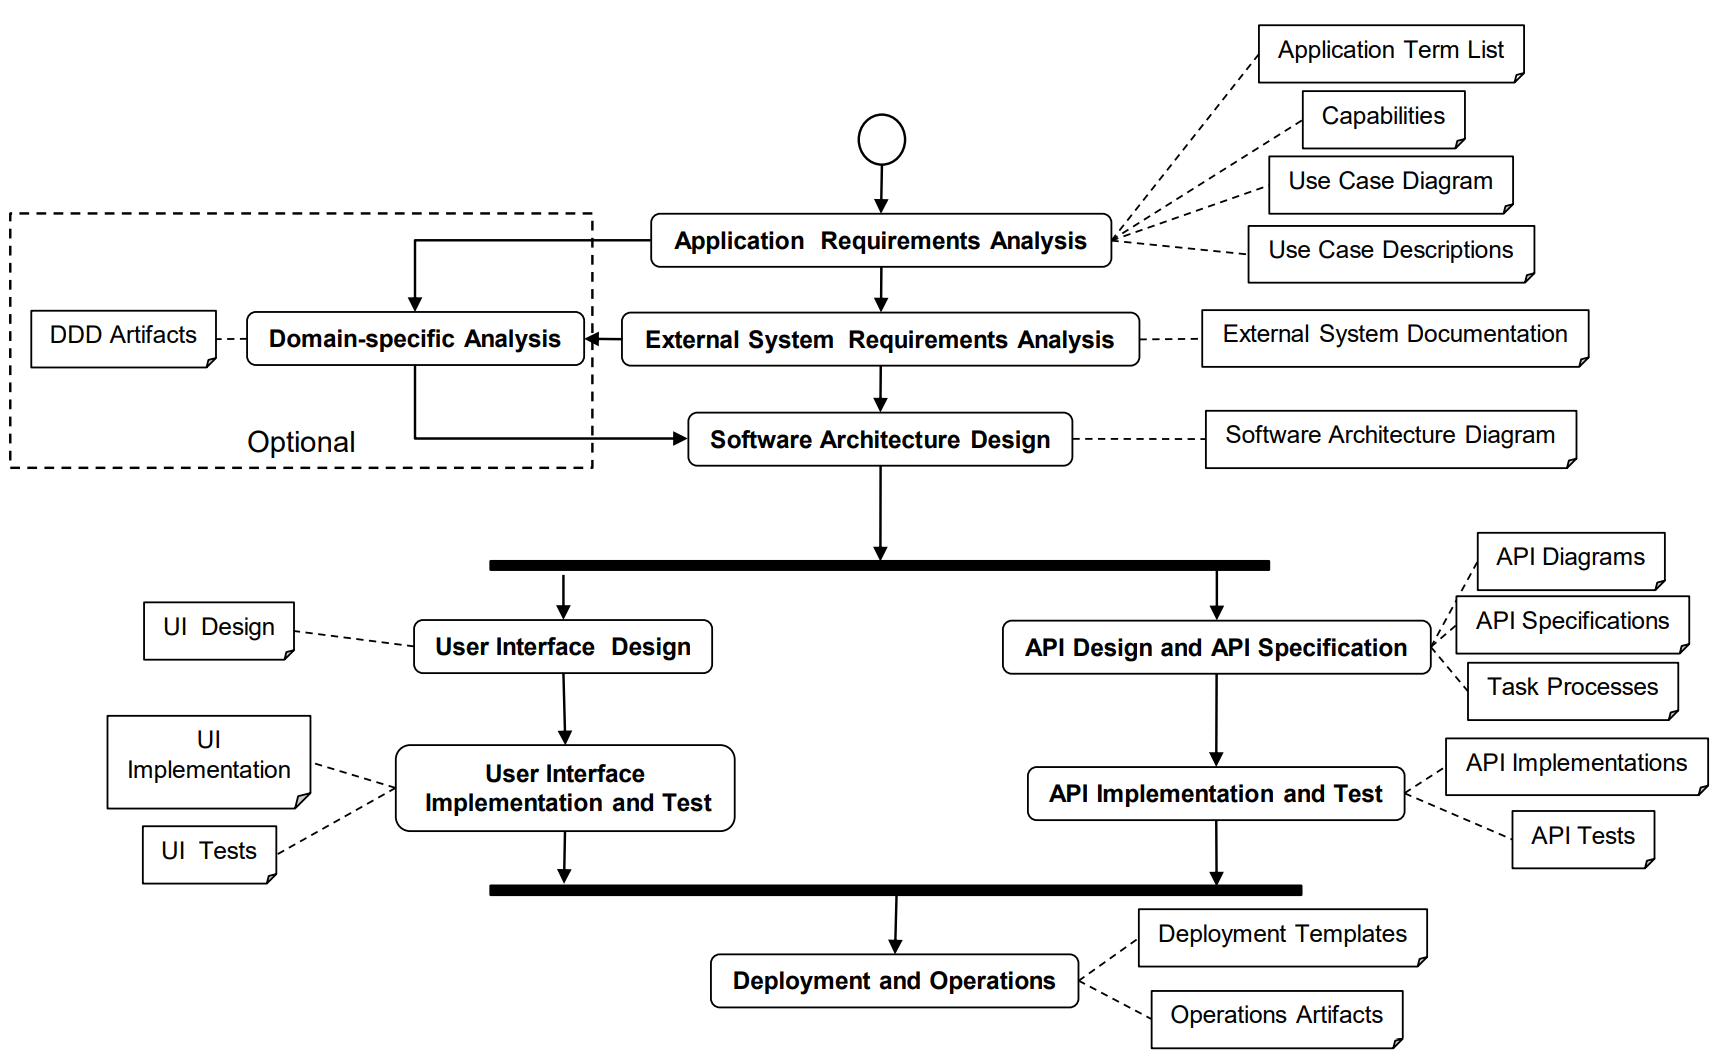
\includegraphics[width=\textwidth]{figures/ume_approach.png}
	\caption{Unified Microservice Engineering Approach \cite{CM-W-OVW}}
	\label{fig:ume_approach}
\end{figure}

\begin{figure}[tb]
	\centering
	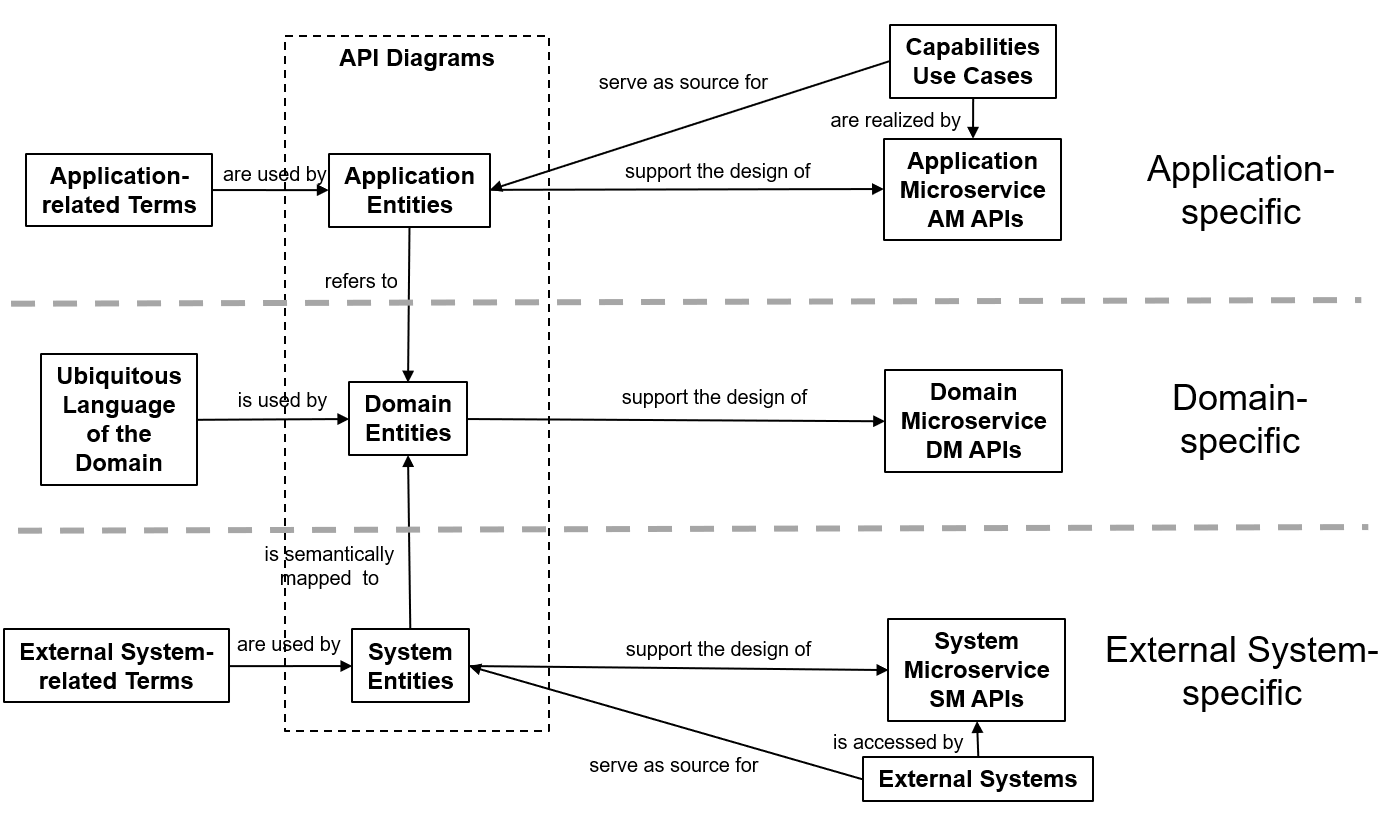
\includegraphics[width=\textwidth]{figures/ume_approach_api_design.png}
	\caption{UME Approach - API Design \cite{CM-W-DES}}
	\label{fig:ume_approach_api_design}
\end{figure}

% \begin{figure}[tb]
% 	\centering
% 	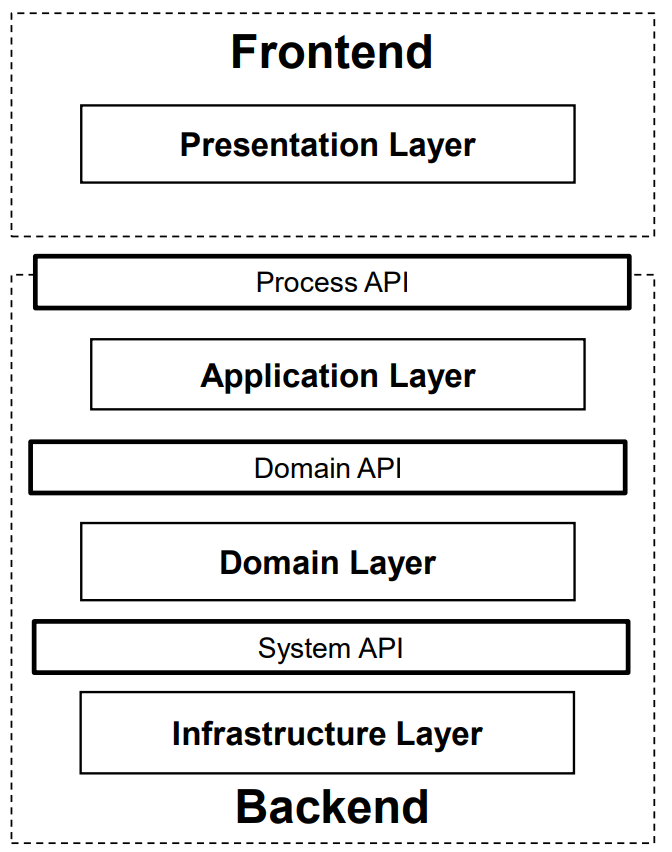
\includegraphics[width=\textwidth]{figures/ume_approach_layers.png}
% 	\caption{UME Approach - Architecture Layers}
% 	\label{fig:ume_approach_layers}
% \end{figure}

% \begin{figure}[tb]
% 	\centering
% 	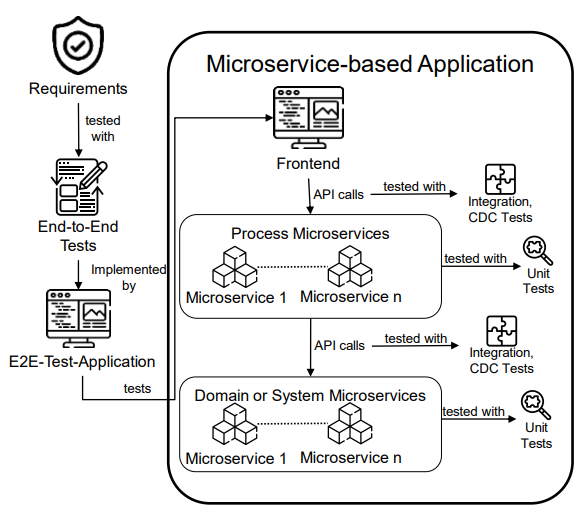
\includegraphics[width=\textwidth]{figures/ume_approach_test_concept.png}
% 	\caption{UME Approach - Test Concept}
% 	\label{fig:ume_approach_test_concept}
% \end{figure}

% \begin{figure}[tb]
% 	\centering
% 	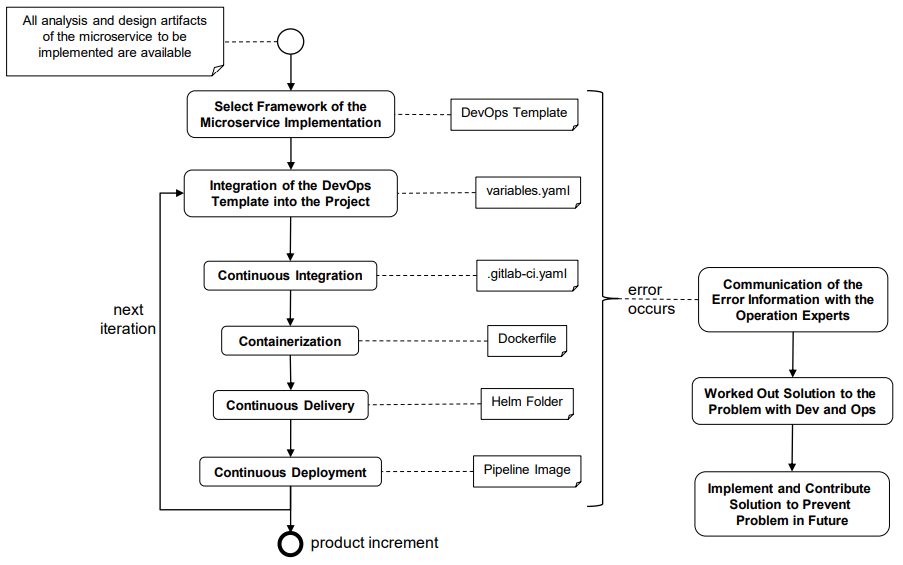
\includegraphics[width=\textwidth]{figures/ume_approach_deployment_operations.png}
% 	\caption{UME Approach - Deployment and Operations}
% 	\label{fig:ume_approach_deployment_operations}
% \end{figure}

% \begin{figure}[tb]
% 	\centering
% 	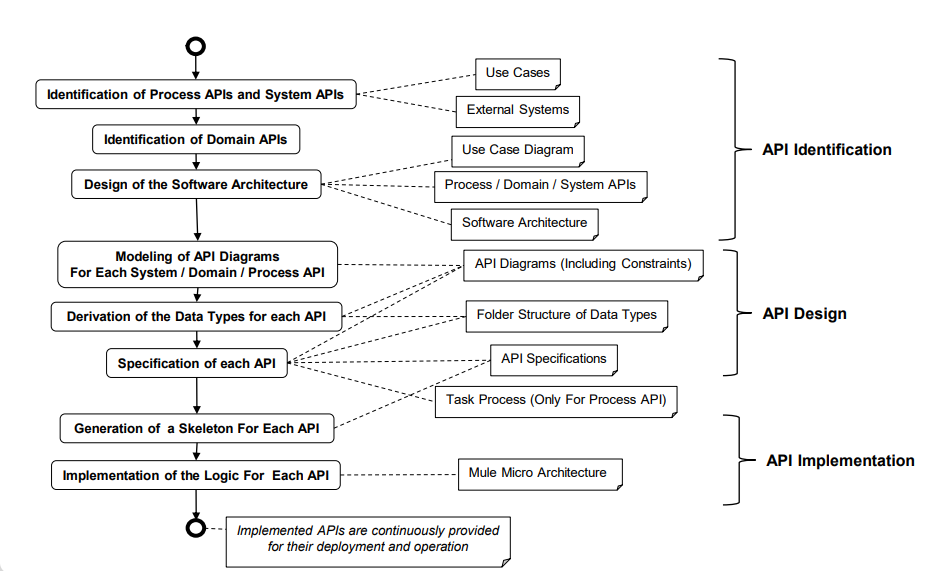
\includegraphics[width=\textwidth]{figures/ume_approach_api_related_actions.png}
% 	\caption{UME Approach - API related Actions}
% 	\label{fig:ume_approach_api_related_actions}
% \end{figure}

% TODO:
% - Software Architecture and System Architecture Diagram
% - Entities and API Design diagram ... also needs more explanation
% - API Diagram to API spec maybe with diagram but might be too much

The Unified Microservice Engineering (UME) approach is a software engineering
process developed by C\&M for the development of applications based on microservices.
An overview of the whole approach can be seen in Figure \ref{fig:ume_approach}.
It is based on two different approaches CMEng and MuleEng,
which were previously developed by C\&M.

% TODO: maybe something about CMEng and MuleEng?

The UME approach consists of four phases: Analysis, Design, Implementation and Test,
and Deployment and Operation. The approach can optionally be extended with domain-driven aspects.

The analysis phase starts with the Application Requirements Analysis
which analyzes and describes the requirements of the application that is to be developed.
This consists of creating an Application Term List which specificies the meaning
of application related terms for all involved parties. The Application Term List
is not a ubiquitous language as it is used in domain-driven design (DDD) because it
may span multiple different domains. Contrary, the ubiquitous language of DDD is always
specific to a single domain. Using the terms from the Application Term List,
capabilities and use cases are defined for the application. 
For each capability a separate use case diagram is created.
The use cases from each use case diagram are further specified in use case descriptions.
Optionally, the Application Requirements Analysis may be extended with additional artifacts
like a business vision and goals or an application sketch.
The standard analysis phase of the UME approach is concluded with the External System Requirements Analysis.
This analysis focues on specifying the requirements for external systems which will be used
by the application. Examples for such external systems are databases, enterprise applications,
and business services. The results of this analysis are documented in the External System Documentation.
In the case that the UME approach is extended with domain-driven aspects,
the analysis phase consists of an additional step: the Domain-specific Analysis.
This step encapsulates the standard DDD and its artifacts like ubiquitous languages
and domain models. % TODO: rewrite The addition of domain-driven aspects is useful when
% the application has to interact with services which may be used by multiple applications.
% In this case, the DDD Artifacts are used to construct Domain APIs which provide a layer
% of abstraction.

% TODO: Grafik für die verschiedenen API Schichten
% FIXME: are these still the right terms for the APIs
After the analysis phase comes the design phase which starts with the Software Architecture Design.
The software architecture of the application consists of Process, System, optional Domain, and Experience APIs.
The Process APIs are derived from use cases and directly provide the functionality set forth
by the use cases. There is a one-to-one mapping between methods of the Process APIs and the use cases.
System APIs are designed to integrated external systems into the application.
The optional Domain APIs provide domain-specific logic as a layer of abstraction
on top of the System APIs. Lastly, the Experience APIs
bridge the gap between the Process APIs which provide the logical functionality needed by
the application and its user interfaces. Different user interfaces may require
different forms of communication or data formats. For this reason, Experience APIs
are used as a layer of abstraction above the Process APIs with one Experience API
per user interface.
Note that during this design step, no specifications for the different APIs are created.
Instead the Software Architecture Design considers each API as a separate service
and constructs an architecture on how to arrange these services.
This is documented in a SystemPlusSoftware Architecture Diagram which is a type of UML
diagram developed by C\&M. % TODO: Explain SPS % A SystemPlusSoftware Architecture Diagram combines
% the physical and logical view of a system into a single diagram by combining
% UML Deployment Diagrams
After the design of the Software Architecture, the UME approach splits into two processes.
One for the user interfaces and one for the APIs.
Firstly, the APIs are designed and specifications are written for them.
The design of the API starts by creating API diagrams which model the entities relevant
for an API and their relationships to other APIs. Each type of API has a separate
type of API diagram and entities. There are Process API diagrams for Process APIs,
Domain API diagrams for Domain APIs, and System API diagrams for System APIs.
These diagrams consist, respectively, out of Process Entities, Domain Entities,
and System Entities. The relation between these entities, APIs and analysis artifacts
can be seen in Figure \ref{fig:ume_approach_api_design}.

Following the design of both the user interfaces and APIs,
the implementation and test phase starts in which all the APIs and user interfaces
are implemented according to their design. To ensure their correctness,
tests are also created. These tests consist of unit tests, integration tests and end-to-end tests.
Unit tests are written to ensure the correctness of single functions.
Integration tests then combine multiple functions together to test a complete API or user interface.
Finally, end-to-end tests verify the correctness of the whole application.
After the implementation and test phase, the two separate processes for the user interfaces
and APIs merge into a single process again. This starts the last phase: deployment and operations.
For the deployment of APIs and user interfaces, so called DevOps Templates are used
which can be reused across different projects. Configurable DevOps Templates reduce the complexity
of deployments because a certain variant of a deployment, like deploying a Go microservice
to a Kubernetes with Helm, only has to be created once and can then be reused with
the right configuration changes for other deployments.

\section{Monitoring in the DevOps Cycle}

% TODO: Do

% As Ebert et al. \cite{EG+16} note, the research into DevOps is primarily concerned with
% building and deploying software. But as the name implies, DevOps is also concerned with the
% operation of software.

The classical software engineering process consists of analysis, design, implementation, testing, and maintenance.
This process is also known as the waterfall model. Developing software with the waterfall model starts
with analyzing the requirements of the complete application. These requirements are then used to design
an application that fulfills them. After the complete application has been designed, it is implemented.
Once the implementation is done, the application is tested to ensure that it fulfills all requirements.
When the testing is completed, the application is shipped to the customer. During the usage of the developed application,
external factors may change which force the application to be updated. This is the last step in the waterfall model
and is referred to as maintenance. In the waterfall model, this is the only phase when errors from previous phases can be corrected
as the waterfall model does not provide the ability to, for example, go back to the design phase during the implementation
to correct mistakes. This process has proven too rigid for most practical software developments.
DevOps (Development and Operations) addresses this problem by adapting the waterfall model from a linear process
into a cycle-based process.
% DevOps (Development and Operations) addresses this rigidity problem of the waterfall model by adopting agile
% business practices. Instead of splitting the development process into the phases of analysis, design, implementation,
% testing, and maintenance, DevOps splits the development process into phases where each phase is meant to complete a sub-set
% of features of the application. These phases are k
The DevOps cycle consists of eight steps. These steps are planning, implementation, building, testing,
releasing, deploying, operating, and monitoring \cite{CM-W-DEV}.
Planning combines the steps of analysis and design from the waterfall model.
In between the phases of implementation and testing from the waterfall model, the DevOps cycle inserts
an additional step called building. In the build step, the source code and artifacts of the application
are combined into a form that can be used by a customer, for example, an executable. Once the application
has been built, the testing step takes place that mirrors the testing phase from the waterfall model.
After the application has been tested, it is shipped to the customer which is turned into an explicit step called releasing
in the DevOps cycle. The DevOps cycle also adds the step of deploying which refers to the setup and installation of an application's release.
Once the application has been deployed, it has to be operated. % TODO: operating
While the application is being used, the monitoring step takes place. In this step,
the application is monitored to find issues that arise during the application's usage.
In the case that issues are found in the application, the DevOps cycle can be restarted from the beginning
to address these issues. This is the cyclic nature of the DevOps cycle in comparison with the linear waterfall model.

% TODO: figure of cycle



% TODO: Connection operation and observability

\section{Integrating Monitoring into the Unified Microservice Engineering Approach}

% TODO: Do

Monitoring is a part of observability and as such should also be considered in DevOps processes.

% TODO: Intro
% - assumptions
% - main part is metric definition -> the rest is just the realization of capturing the metrics

\begin{figure}[tb]
	\centering
	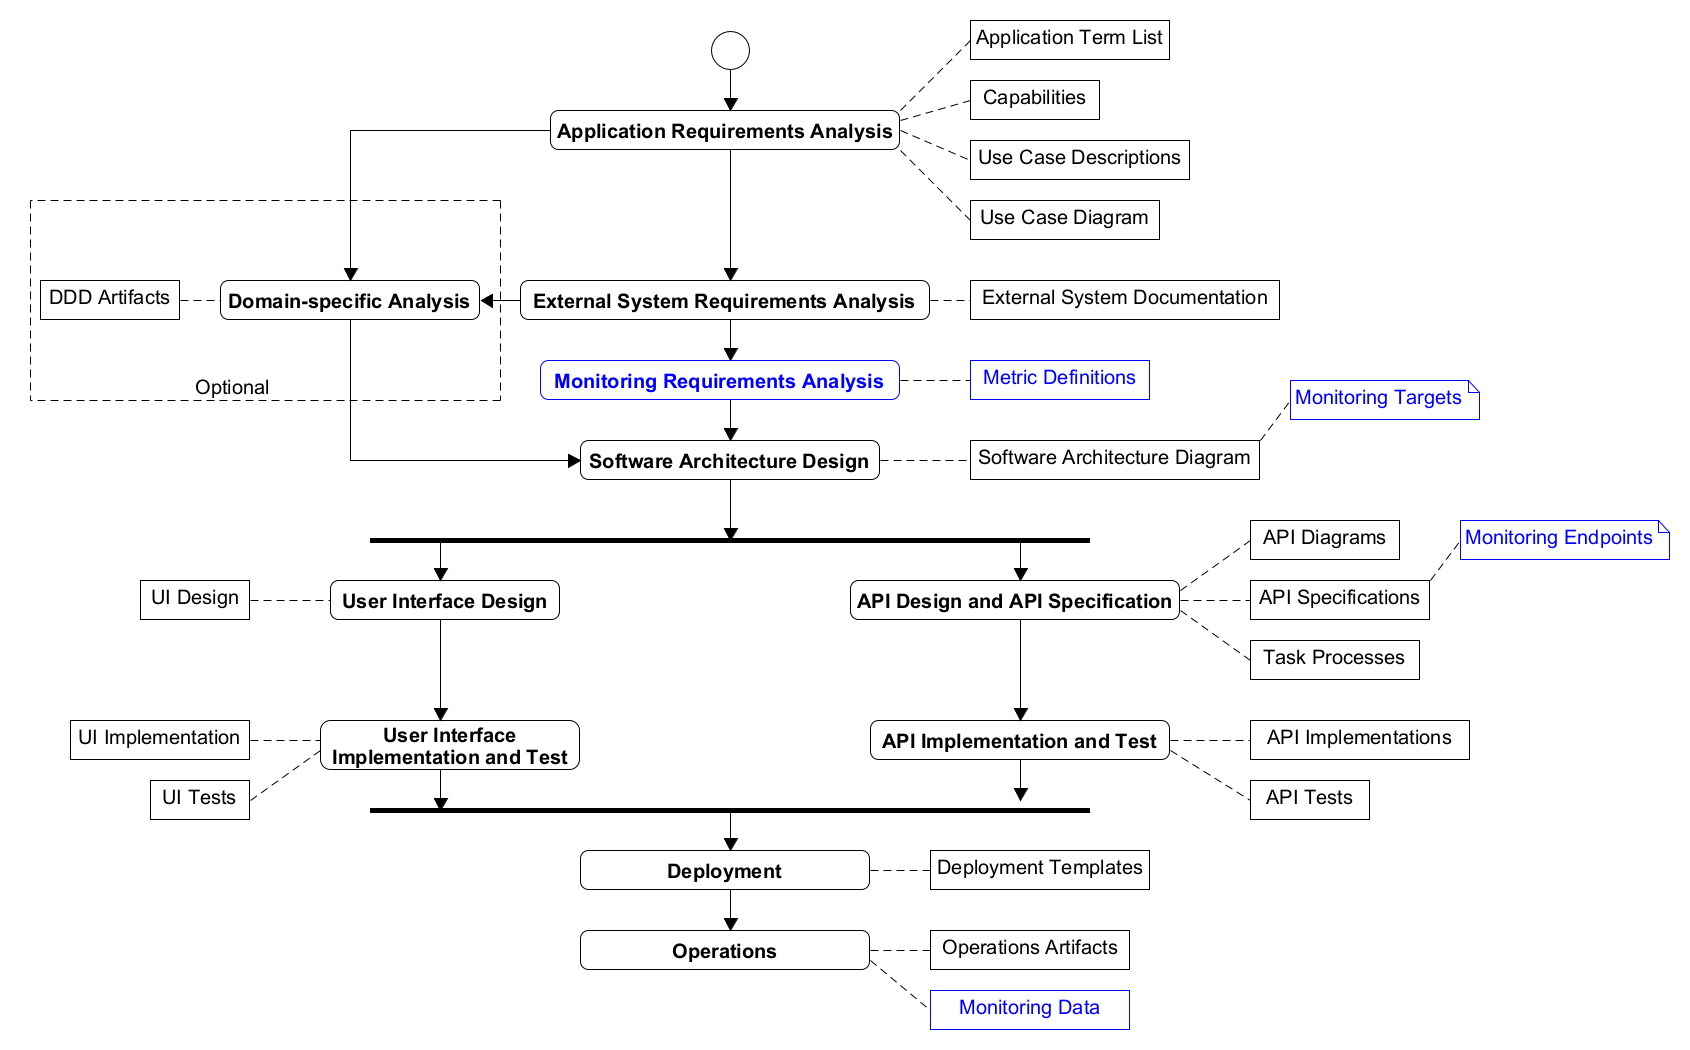
\includegraphics[width=\textwidth]{figures/ume_approach_extended.png}
	\caption{Extended Unified Microservice Engineering Approach}
	\label{fig:ume_approach_extended}
\end{figure}

% TODO: Assumptions
% - pull based
% - monitoring system already exists
% - monitoring system is capable of aggregating raw values
The extension of the UME approach with a monitoring concept is based on two assumptions.
The first assumption is that a viable monitoring system already exists. This assumption
is made because it simplifies the step API Design and API Specification in the extended UME approach.
% TODO: besser formulieren
% During this step the API of microservice, that provide data to the monitoring system, is specified
% and must include a monitoring endpoint for collecting the data from the microservice. If the monitoring system
% would not already exist at this point, the API of the microservice could not be specified because
% the API specification requires knowledge about the format of data that is used by the monitoring system.

% TODO: finish
The second assumption is that the monitoring system works by pulling data from the application
as opposed to the data being sent to the monitoring system by the application. This assumption
is mainly based on the API-oriented approach to designing microservices taken by the UME approach.
% TODO:
% In this way, the API of microservices that provide data to the monitoring system
% can be explicitly extended by a monitoring endpoint 

% TODO: Figure for monitoring targets being marked in a software architecture diagram

The extended UME approach can be seen in Figure \ref{fig:ume_approach_extended}.
The extension of the UME approach with a monitoring concept starts in the analysis phase
of the development process. After the Application Requirements Analysis and External System Requirements Analysis,
a new analysis called Monitoring Requirements Analysis is added. The goal of this analysis
is the creation of an artifact called Metric Definitions. The Metric Definitions artifact is a list
that contains the definition of all metrics that should be monitored.
The definition of each metric consists of the metric's name, the purpose of the metric,
its type, a list of values necessary for calculating the metric, how the metric should
be represented visually and optionally different ranges of values of the metric with associated
state information. An example of a metric definition can be seen in Listing \ref{lis:metric_definition_example}.
The purpose of a metric should clarify the meaning of a metric.
An example of this comes from the manufacturing industry where the OEE (Overall Equipment Effectiveness)
metric measures the percentage of planned production time that is truly productive.
Additionally, the purpose of a metric should state what the metric is being used for.
Continuing with the example of the OEE metric, the purpose would be to identify bottlenecks
in production chains and to improve productivity.
A metric can be categorized by the type of information that it provides and how it is calculated.
A metric is either a business metric or a technical metric and its method of calculation is either
elementary or through aggregation.
Business metrics capture the performance of business processes.
An example from BestRentalPoC is the number of issued digital driving licenses.
Technical metrics capture the state of the application as numerical values.
Examples of technical metrics are the four golden signals Latency, Traffic, Errors, and Saturation
as defined in Chapter \ref{cha:foundations}.
An elementary metric can be calculated from a single value captured from the application and does not
need any other information. Elementary metrics can be combined to form aggregated metrics
which are calculated by combining the values of different elementary metrics into a single value.
The list of values necessary for calculating the metric is used in a later step
of the extended UME approach to define monitoring targets in the software architecture of the application.
If the type of a metric is elementary then the list of values necessary for calculating the metric
must consist of exactly one entry. If the metric is aggregated then the list of values necessary for calculating
the metric should also state how the different values in the list are combined to form the aggregated metric.
The visual representation should describe how the metric can be presented in the chosen monitoring tool.
This description should be kept short. An example of such a description can be seen in Listing \ref{lis:metric_definition_example}.
Optionally, a metric's definition can contain value ranges that signal different states of a metric.
Taking the metric Latency, possible value ranges would be: <1ms means Latency is Good, <10ms means High Latency,
and >1s means Critical Latency. These states can then be used to, for example, trigger alerts or start
processes. For example, if the metric Latency reaches the state of Critical Latency in a cloud application,
a process that might be started is to scale the application horizontally by adding more instances of services.

\begin{figure}[tb]
\begin{lstlisting}[caption = {Example of a Metric Definition}, label = {lis:metric_definition_example}, style = kit-cm, language=]
Name: Service A Memory Usage

Purpose:
Capture the amount of main memory being used by Service A
to identify memory leaks in the service's implementation.

Type: Elemental, Technical

Values:
- Service A: currently used main memory in bytes.

Visual Representation:
- Option A: Line Graph with time as the x-axis and the current metric value as the y-axis.
- Option B: Gauge with different colors for the different ranges of the metric.

Ranges:
- Ok: Value < 100 MB
- Warning: 100 MB < Value < 500 MB
- Critical: Value > 500 MB
\end{lstlisting}
\end{figure}

The next adaptation of the UME approach is in the Software Architecture Design.
The main artifact of the Software Architecture Design is the Software Architecture Diagram.
The C\&M research group uses SPS (SystemPlusSoftware) diagrams for this purpose.
Based on the metrics defined during the Monitoring Requirements Analysis,
microservices within the Software Architecture Diagram are optionally marked as monitoring targets.
A monitoring target is a microservice that can provide values that are listed in a metric's definition.
% TODO: es sollte da durch klar sein wo daten her kommen können während dem design
% Based on the capabilities defined in the Application Requirements Analysis
% and the External System Documentation from the External System Requirements Analysis,

The next change to the UME approach is the extension of the API specifications created during the
API Design and API Specification step. Microservices that have been marked as monitoring targets
during the Software Architecture Design need to include monitoring endpoints in their API
through which the data that is being collected by the microservice can be collected by the monitoring system.
Because the assumption was made the monitoring system is chosen in advance,
the monitoring endpoint in the API specification can be designed to fit the monitoring system.

The last change to the UME approach is the addition of a new artifact to the Operations step.
The new artifact is the data that is being collected by the monitoring system from the application
and is called monitoring data. The monitoring data includes both the raw values being collected
from the application as well as the values of the metrics that have been defined.

% TODO: wieso passt das zu DevOps?
% - everything can be adapted on the fly